\documentclass[10pt]{article}
\usepackage[a4paper, margin=1.5cm, landscape]{geometry}
\usepackage{tikz}
\usepackage{xcolor}
\usepackage{ulem} % For the strikethrough text
\usetikzlibrary{positioning, fit, calc, backgrounds, arrows.meta, shapes.multipart, decorations.pathreplacing}

% Define the color palette based on your spec
\definecolor{boxyellow}{HTML}{FFFDE7}
\definecolor{borderyellow}{HTML}{FFF3CD}
\definecolor{boxblue}{HTML}{E3F2FD}
\definecolor{borderblue}{HTML}{BBDEFB}
\definecolor{boxred}{HTML}{FFEBEE}
\definecolor{borderred}{HTML}{FFCDD2}
\definecolor{boxgreen}{HTML}{E8F5E9}
\definecolor{bordergreen}{HTML}{C8E6C9}
\definecolor{boxpurple}{HTML}{F3E5F5}
\definecolor{borderpurple}{HTML}{E1BEE7}
\definecolor{boxgray}{HTML}{FAFAFA}
\definecolor{bordergray}{HTML}{E0E0E0}

\begin{document}
\begin{center}
% Using resizebox to ensure it fits the page width beautifully
\resizebox{1.0\textwidth}{!}{
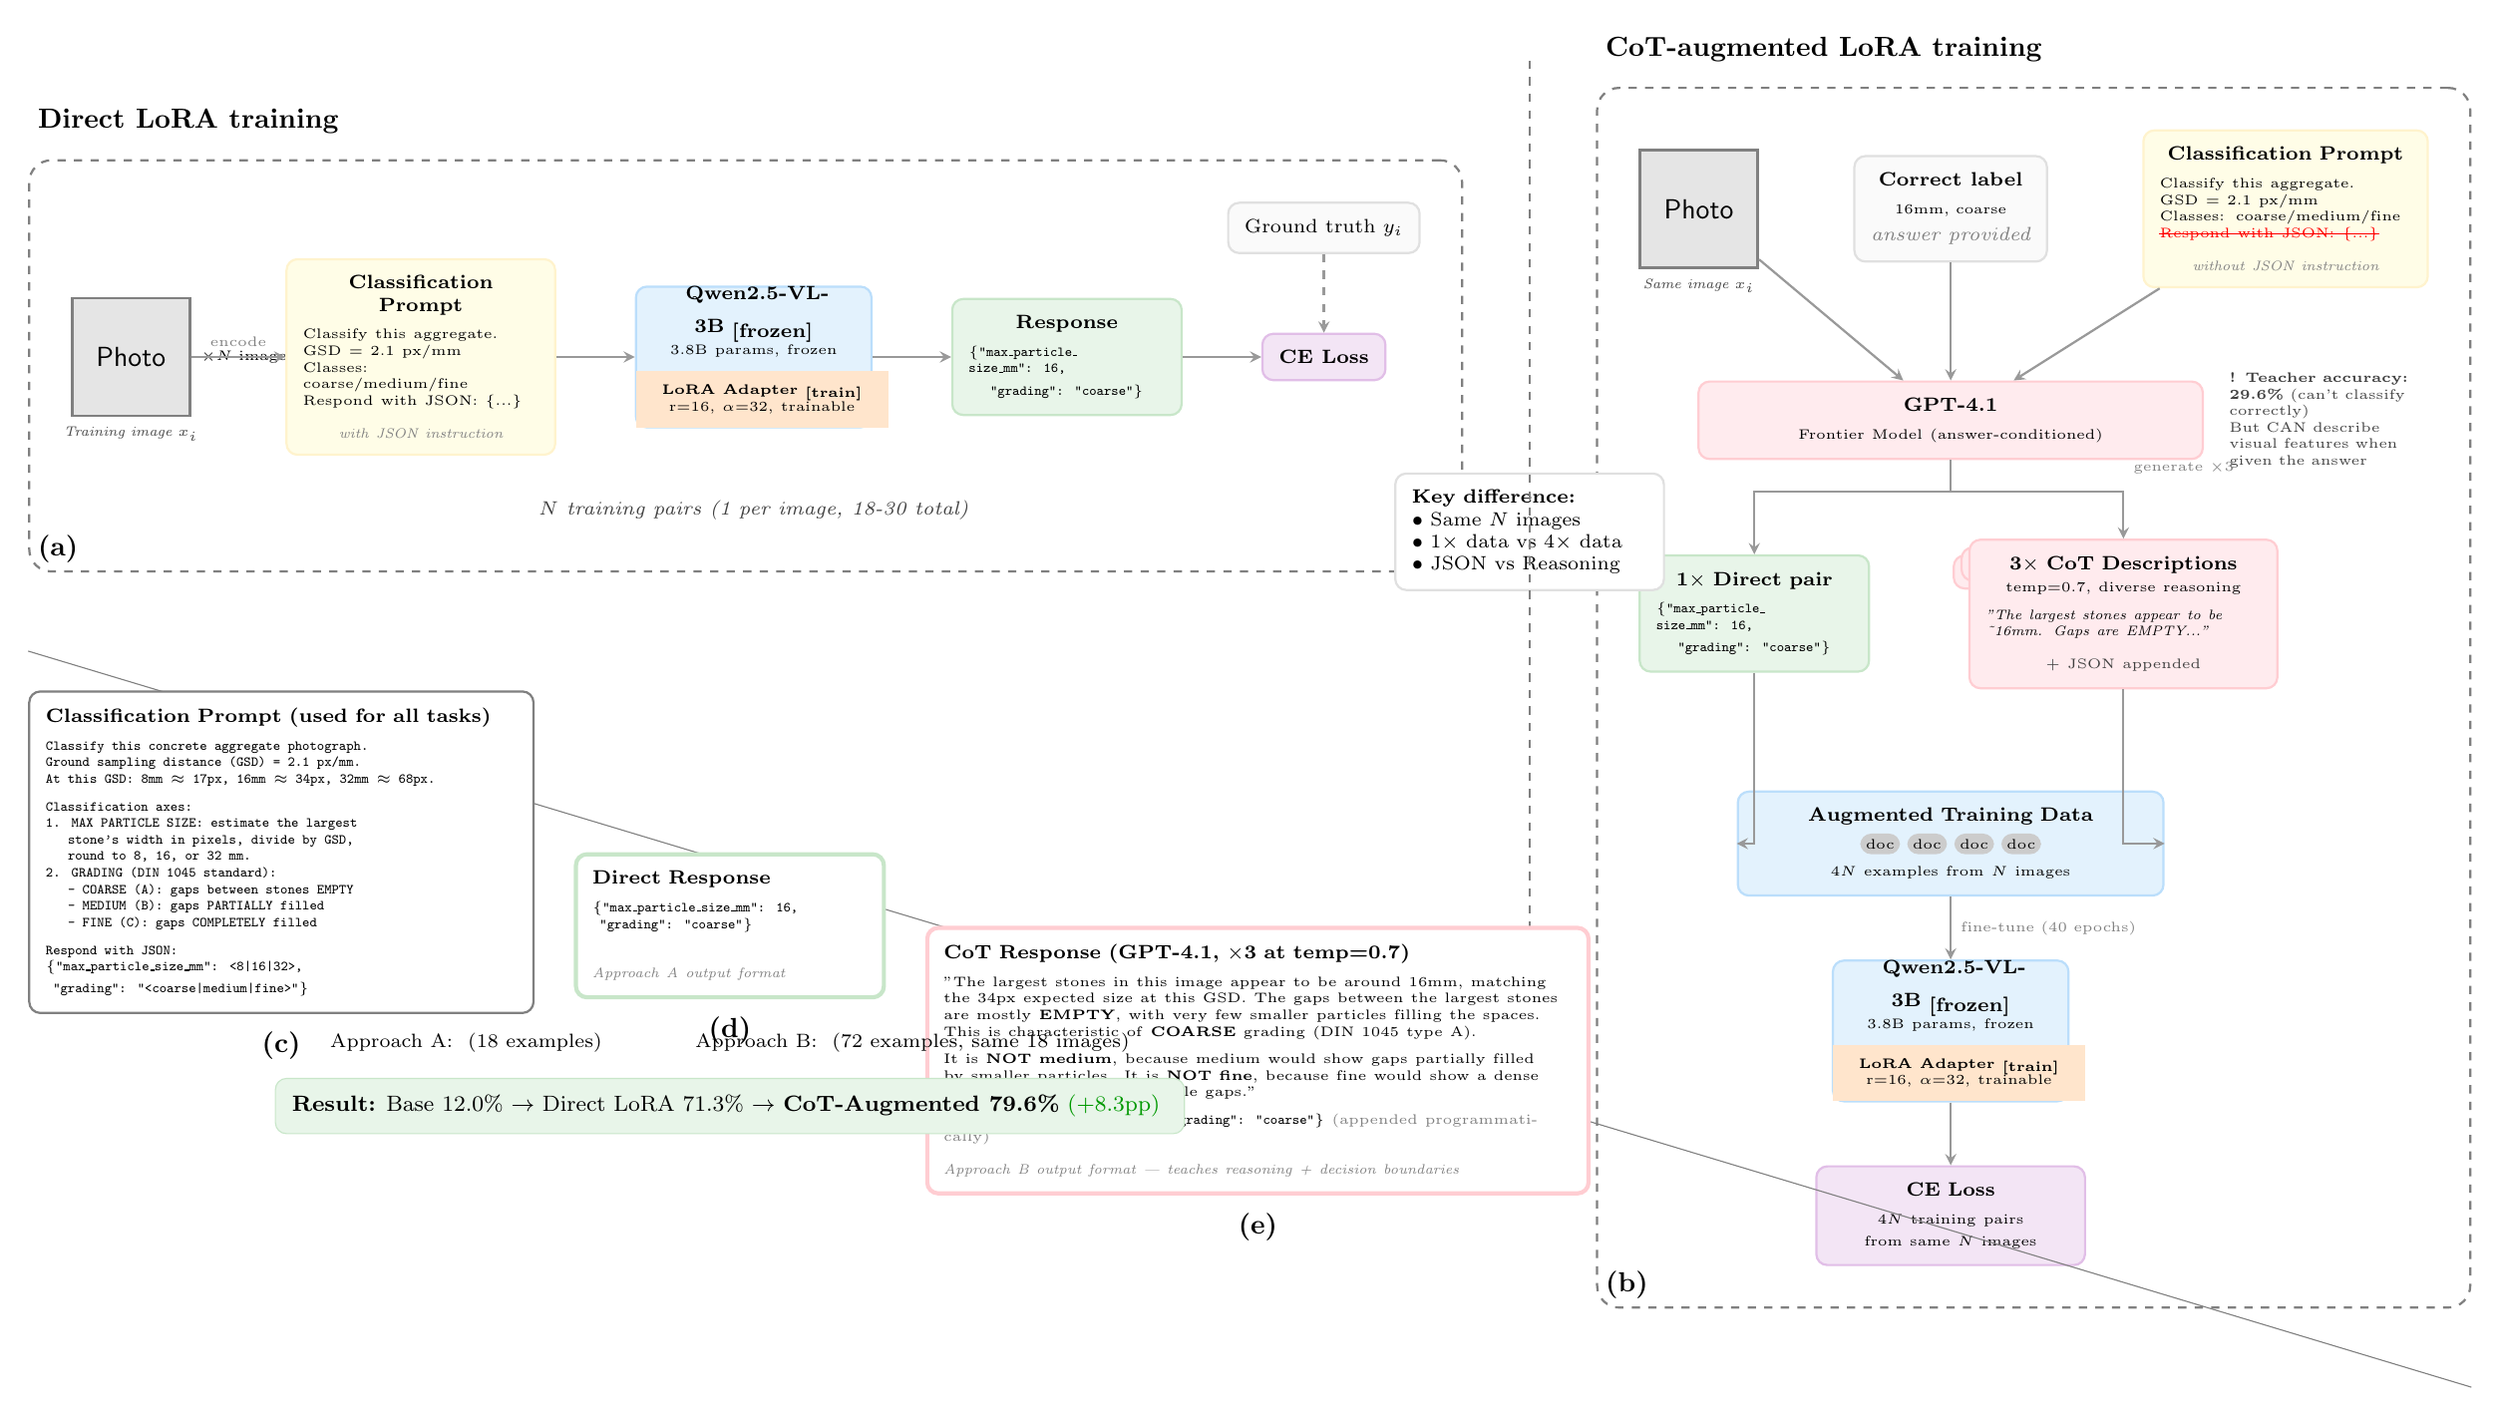
\begin{tikzpicture}[
    font=\sffamily,
    % Base styles for boxes
    basebox/.style={rectangle, rounded corners=4pt, draw, align=center, font=\scriptsize, inner sep=6pt, line width=0.8pt},
    yellowbox/.style={basebox, fill=boxyellow, draw=borderyellow},
    bluebox/.style={basebox, fill=boxblue, draw=borderblue},
    redbox/.style={basebox, fill=boxred, draw=borderred},
    greenbox/.style={basebox, fill=boxgreen, draw=bordergreen},
    purplebox/.style={basebox, fill=boxpurple, draw=borderpurple},
    graybox/.style={basebox, fill=boxgray, draw=bordergray},
    whitebox/.style={basebox, fill=white, draw=gray!50, align=left},
    % Arrow styles
    arr/.style={->, >=stealth, draw=gray!80, thick},
    dasharr/.style={->, >=stealth, draw=gray!80, thick, dashed},
    % Grouping box styles
    dashedgroup/.style={rectangle, rounded corners=8pt, draw=gray, dashed, inner sep=15pt, line width=0.8pt}
]

% =======================================================
% TOP-LEFT: (a) Direct LoRA Training
% =======================================================

% 1. Training Image (Placeholder for sample_A16.jpg)
\node[draw=gray, line width=1px, minimum size=1.5cm, fill=gray!20, label={[font=\tiny\itshape\color{darkgray}]below:Training image $x_i$}, label={[font=\tiny]right:$\times N$ images}] (imgA) {Photo};

% Uncomment line below and remove node above when compiling with your image
% \node[draw=gray, line width=1px, inner sep=0pt, label={[font=\tiny\itshape\color{darkgray}]below:Training image $x_i$}] (imgA) {\includegraphics[width=1.5cm, height=1.5cm]{images/sample_A16.jpg}};

% 3. Prompt Box
\node[yellowbox, right=1.2cm of imgA, text width=3cm] (promptA) {
    \textbf{Classification Prompt}\\[4pt]
    \raggedright \tiny
    Classify this aggregate.\\
    GSD = 2.1 px/mm\\
    Classes: coarse/medium/fine\\
    Respond with JSON: \{...\}\\[4pt]
    \raggedleft \textit{\color{gray}with JSON instruction}
};

% 5. Model Block
\node[bluebox, right=1cm of promptA, text width=3cm, inner sep=0pt] (modelA) {
    \vspace{4pt}
    \textbf{Qwen2.5-VL-3B \raisebox{-0.5ex}{[frozen]}}\\
    \tiny 3.8B params, frozen\\[4pt]
    \colorbox{orange!20}{\parbox{\linewidth}{\centering \vspace{2pt}\textbf{LoRA Adapter \raisebox{-0.5ex}{[train]}}\\ \tiny r=16, $\alpha$=32, trainable\vspace{2pt}}}
};

% 7. Output Box
\node[greenbox, right=1cm of modelA, text width=2.5cm] (outA) {
    \textbf{Response}\\[4pt]
    \raggedright \ttfamily \tiny
    \{"max\_particle\_\\
    size\_mm": 16,\\
    "grading": "coarse"\}
};

% 9. Loss Box
\node[purplebox, right=1cm of outA] (lossA) {\textbf{CE Loss}};

% 10. Label Box
\node[graybox, above=1cm of lossA] (labelA) {Ground truth $y_i$};

% Arrows for (a)
\draw[arr] (imgA) -- node[above, font=\tiny\color{gray}] {encode} (promptA);
\draw[arr] (promptA) -- (modelA);
\draw[arr] (modelA) -- (outA);
\draw[arr] (outA) -- (lossA);
\draw[dasharr] (labelA) -- (lossA);

% Annotations & Grouping for (a)
\node[below=0.8cm of modelA, font=\itshape\scriptsize\color{darkgray}] (annA) {$N$ training pairs (1 per image, 18-30 total)};
\node[dashedgroup, fit=(imgA) (promptA) (modelA) (outA) (lossA) (labelA) (annA)] (groupA) {};
\node[above=0.2cm of groupA.north west, anchor=south west, font=\bfseries] {Direct LoRA training};
\node[above right, font=\bfseries] at (groupA.south west) {(a)};

% =======================================================
% TOP-RIGHT: (b) CoT-Augmented LoRA Training
% =======================================================

% Position the entire (b) block to the right of (a)
\coordinate (startB) at ($(groupA.east) + (3cm, 2cm)$);

% 1, 2, 3 Inputs
\node[draw=gray, line width=1px, minimum size=1.5cm, fill=gray!20, label={[font=\tiny\itshape\color{darkgray}]below:Same image $x_i$}] (imgB) at (startB) {Photo};

\node[graybox, right=1.2cm of imgB] (labelB) {
    \textbf{Correct label}\\[2pt] \tiny 16mm, coarse\\[2pt] \textit{\color{gray}answer provided}
};

\node[yellowbox, right=1.2cm of labelB, text width=3.2cm] (promptB) {
    \textbf{Classification Prompt}\\[4pt]
    \raggedright \tiny
    Classify this aggregate.\\
    GSD = 2.1 px/mm\\
    Classes: coarse/medium/fine\\
    {\color{red}\sout{Respond with JSON: \{...\}}}\\[4pt]
    \raggedleft \textit{\color{gray}without JSON instruction}
};

% 5. Frontier Model
\node[redbox, below=1.5cm of labelB, text width=6cm] (gpt) {
    \textbf{GPT-4.1 }\\[2pt]
    \tiny Frontier Model (answer-conditioned)
};
\node[right=0.2cm of gpt, font=\tiny\color{darkgray}, text width=2.5cm] {
    \textbf{! Teacher accuracy: 29.6\%} (can't classify correctly)\\
    But CAN describe visual features when given the answer
};

% 7a. Direct Pair
\node[greenbox, below=1.2cm of gpt, xshift=-2.5cm, text width=2.5cm] (dirB) {
    \textbf{1$\times$ Direct pair}\\[4pt]
    \raggedright \ttfamily \tiny
    \{"max\_particle\_\\
    size\_mm": 16,\\
    "grading": "coarse"\}
};

% 7b. CoT Description (Stacked visual)
\node[redbox, below=1.2cm of gpt, xshift=2cm, text width=3.5cm, fill=boxred, draw=borderred] (cotB3) {};
\node[redbox, below=1.1cm of gpt, xshift=2.1cm, text width=3.5cm, fill=boxred, draw=borderred] (cotB2) {};
\node[redbox, below=1.0cm of gpt, xshift=2.2cm, text width=3.5cm] (cotB1) {
    \textbf{3$\times$ CoT Descriptions}\\[2pt]
    \tiny temp=0.7, diverse reasoning\\[4pt]
    \raggedright \itshape \tiny
    "The largest stones appear to be \textasciitilde 16mm. Gaps are EMPTY..."\\[4pt]
    \raggedleft \upshape \color{darkgray} + JSON appended
};

% 9. Augmented Data Box
\node[bluebox, below=1.5cm of dirB, xshift=2.5cm, text width=5cm] (augB) {
    \textbf{Augmented Training Data}\\
    \vspace{2pt}
    \tikz{\node[fill=gray!40, inner sep=2pt]{\tiny doc};} \tikz{\node[fill=gray!40, inner sep=2pt]{\tiny doc};} \tikz{\node[fill=gray!40, inner sep=2pt]{\tiny doc};} \tikz{\node[fill=gray!40, inner sep=2pt]{\tiny doc};}\\
    \tiny 4$N$ examples from $N$ images
};

% 11. Model B
\node[bluebox, below=0.8cm of augB, text width=3cm, inner sep=0pt] (modelB) {
    \vspace{4pt}
    \textbf{Qwen2.5-VL-3B \raisebox{-0.5ex}{[frozen]}}\\
    \tiny 3.8B params, frozen\\[4pt]
    \colorbox{orange!20}{\parbox{\linewidth}{\centering \vspace{2pt}\textbf{LoRA Adapter \raisebox{-0.5ex}{[train]}}\\ \tiny r=16, $\alpha$=32, trainable\vspace{2pt}}}
};

% 13. Loss B
\node[purplebox, below=0.8cm of modelB, text width=3cm] (lossB) {
    \textbf{CE Loss}\\[2pt]
    \tiny 4$N$ training pairs from same $N$ images
};

% Arrows for (b)
\draw[arr] (imgB) -- (gpt);
\draw[arr] (labelB) -- (gpt);
\draw[arr] (promptB) -- (gpt);
\draw[arr] (gpt.south) -- ++(0,-0.4) -| (dirB.north);
\draw[arr] (gpt.south) -- ++(0,-0.4) -| node[right, font=\tiny\color{gray}, yshift=0.3cm] {generate $\times 3$} (cotB1.north);
\draw[arr] (dirB.south) |- (augB.west);
\draw[arr] (cotB1.south) |- (augB.east);
\draw[arr] (augB) -- node[right, font=\tiny\color{gray}] {fine-tune (40 epochs)} (modelB);
\draw[arr] (modelB) -- (lossB);

% Grouping for (b)
\node[dashedgroup, fit=(imgB) (promptB) (gpt) (cotB3) (lossB)] (groupB) {};
\node[above=0.2cm of groupB.north west, anchor=south west, font=\bfseries] {CoT-augmented LoRA training};
\node[above right, font=\bfseries] at (groupB.south west) {(b)};

% =======================================================
% KEY DIFFERENCE ANNOTATION (Between a and b)
% =======================================================
\node[graybox, fill=white, text width=3cm, align=left, font=\scriptsize] (diff) at ($(groupA.east)!0.5!(groupB.west)$) {
    \textbf{Key difference:}\\
    $\bullet$ Same $N$ images\\
    $\bullet$ 1$\times$ data vs 4$\times$ data\\
    $\bullet$ JSON vs Reasoning
};
\draw[draw=gray, dashed, thick] ($(groupA.east)!0.5!(groupB.west) + (0, 6)$) -- ($(groupA.east)!0.5!(groupB.west) + (0, -6)$);

% =======================================================
% BOTTOM SECTIONS: (c, d, e)
% =======================================================

% Horizontal separator line
\draw[draw=gray, thin] ($(groupA.south west) + (0, -1)$) -- ($(groupB.south east) + (0, -1)$);

% (c) Classification Prompt
\node[whitebox, draw=gray, below=1.5cm of groupA.south west, anchor=north west, text width=6cm] (panelC) {
    \textbf{Classification Prompt (used for all tasks)}\\[4pt]
    \ttfamily\tiny
    Classify this concrete aggregate photograph.\\
    Ground sampling distance (GSD) = 2.1 px/mm.\\
    At this GSD: 8mm $\approx$ 17px, 16mm $\approx$ 34px, 32mm $\approx$ 68px.\\[4pt]
    Classification axes:\\
    1. MAX PARTICLE SIZE: estimate the largest\\
    \ \ \ stone's width in pixels, divide by GSD,\\
    \ \ \ round to 8, 16, or 32 mm.\\
    2. GRADING (DIN 1045 standard):\\
    \ \ \ - COARSE (A): gaps between stones EMPTY\\
    \ \ \ - MEDIUM (B): gaps PARTIALLY filled\\
    \ \ \ - FINE (C): gaps COMPLETELY filled\\[4pt]
    Respond with JSON:\\
    \{"max\_particle\_size\_mm": <8|16|32>,\\
    \ "grading": "<coarse|medium|fine>"\}
};
\node[below=0.1cm of panelC, font=\bfseries] {(c)};

% (d) Direct Response
\node[whitebox, draw=bordergreen, line width=1.5pt, right=0.5cm of panelC, anchor=north west, text width=3.5cm] (panelD) {
    \textbf{Direct Response}\\[4pt]
    \ttfamily\tiny
    \{"max\_particle\_size\_mm": 16,\\
    \ "grading": "coarse"\}\\[10pt]
    \normalfont\color{gray} \itshape Approach A output format
};
\node[below=0.1cm of panelD, font=\bfseries] {(d)};

% (e) CoT Response
\node[whitebox, draw=borderred, line width=1.5pt, right=0.5cm of panelD, anchor=north west, text width=8cm] (panelE) {
    \textbf{CoT Response (GPT-4.1, $\times$3 at temp=0.7)}\\[4pt]
    \tiny
    "The largest stones in this image appear to be around 16mm, matching the 34px expected size at this GSD. The gaps between the largest stones are mostly \textbf{EMPTY}, with very few smaller particles filling the spaces. This is characteristic of \textbf{COARSE} grading (DIN 1045 type A).\\[4pt]
    It is \textbf{NOT medium}, because medium would show gaps partially filled by smaller particles. It is \textbf{NOT fine}, because fine would show a dense packed texture with no visible gaps."\\[4pt]
    \ttfamily
    + \{"max\_particle\_size\_mm": 16, "grading": "coarse"\} \normalfont\color{gray}(appended programmatically)\\[4pt]
    \normalfont\color{gray} \itshape Approach B output format --- teaches reasoning + decision boundaries
};
\node[below=0.1cm of panelE, font=\bfseries] {(e)};

% =======================================================
% BOTTOM RESULTS BANNER
% =======================================================
\node[fill=boxgreen, draw=bordergreen, rounded corners=4pt, align=center, font=\footnotesize, inner sep=6pt, below=1cm of panelD] (results) {
    \textbf{Result:} Base 12.0\% $\rightarrow$ Direct LoRA 71.3\% $\rightarrow$ \textbf{CoT-Augmented 79.6\%} {\color{green!60!black}(+8.3pp)}
};

% Data Multiplier Visualization
\node[above=0.2cm of results, font=\scriptsize] {
    Approach A: \textcolor{gray}{$\blacksquare$} (18 examples) \hspace{1cm}
    Approach B: \textcolor{blue!60}{$\blacksquare\blacksquare\blacksquare\blacksquare$} (72 examples, same 18 images)
};

\end{tikzpicture}
}
\end{center}
\end{document}



